% !TEX root = ../maturaarbeit.tex
\chapter{Training the Agent}\label{chap:training}
In this chapter I will cover the results of training agents in the "Soccer" environment and it's variations. Further I will discuss some of the aspects of training an agent in general, presented on the example of my specific environment, therein providing an answer for my original research question.
\nolinebreak 
% How can a DRL algorithm be trained to choose optimal actions in an environment and how can its performance be influenced and improved?
% Wie Lässt sich ein DRL Algorithmus trainieren optimale Aktionen in einer Umgebung zu wählen und wodurch lässt sich seine Leistung beeinflussen und verbessern?
\section{Baseline Results}\label{sec:tr:baseline_results}

\begin{figure}[H]
    \centering
    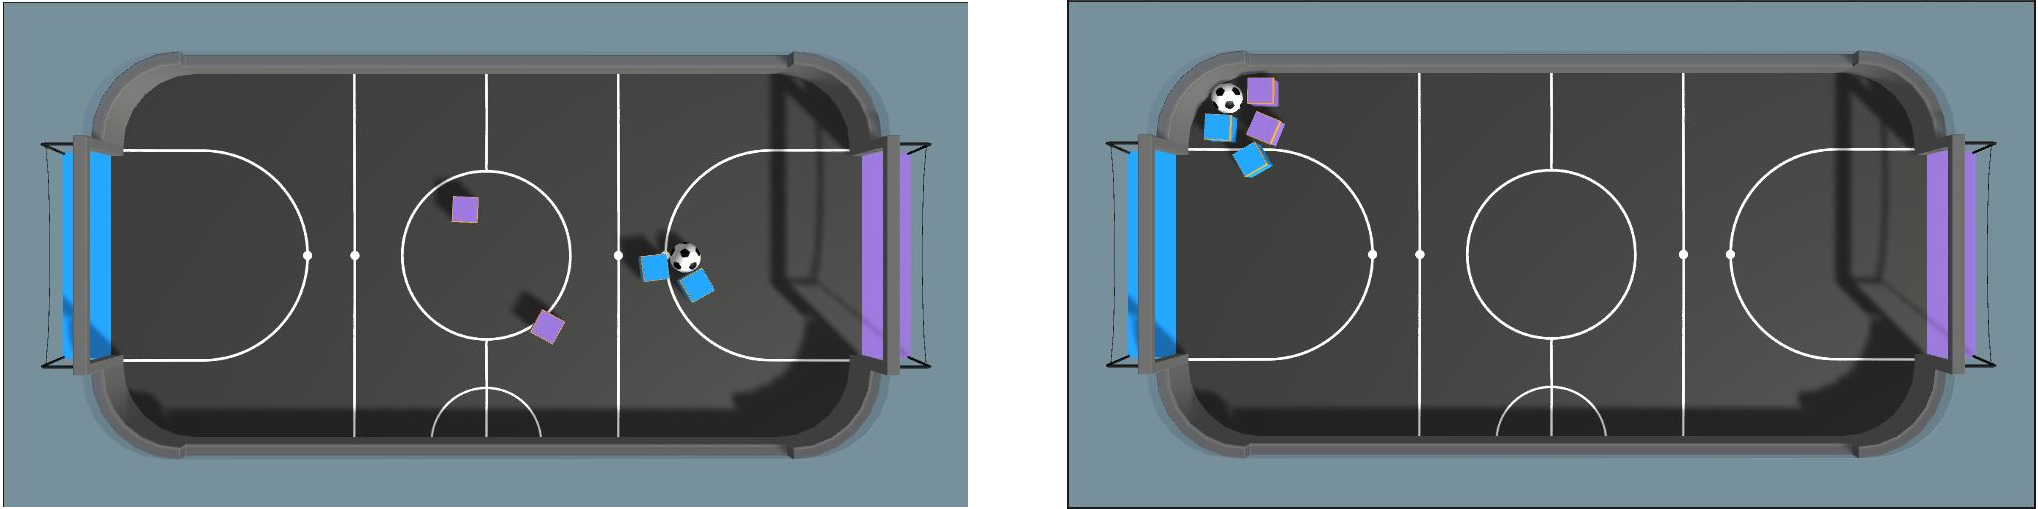
\includegraphics[width=0.7\linewidth]{figures/baseline.png}
    \caption{Illustration of playing behaviour}
    \label{fig:base_returns}
\end{figure}
% initally random stuff
\noindent
Baseline training was fairly successful. Performance of the learned policy exceeded expectations, leading to real gameplay. When observing play on inference, a few behavioural become apparent. When the ball rolls towards an agent's own goal it tend's to push it to the side, sometimes bouncing it of the rounded corner, to the other side of the playing field, from where it may proceed to "counter". 
\\ Generally, the agents seem to have learned a very aggressive "ball chasing" behaviour, which sometimes leads to pushing the ball in to their own goal in an attempt to catch up to it. Further if both agents of one team are close to the ball, they display "infighting" behaviour, which often leads to the ball being lost instead of a goal being scored.
\\At times agents also get the ball stuck in corners. I am uncertain if this is exploitative behaviour, hitting it repeatedly could lead to much higher return values than scoring goals. I think most these patterns may be the result of too high a reward for touching the ball. 

% improved 
% 1-2 strategies
\section{Parallelization}\label{sec:tr:parallel}
In the "Soccer" environment the operation time of \code{UnityEnvironment.step()} is relatively high, leading to roughly 90\% of training time being spent waiting for it to return. Because f this higher degrees of parallelization  are needed. By default, in the baseline environment 32 agents are already trained in parallel. However increasing this number only seemed to increase execution time further. The suggestion of increasing simulation speed proposed in \cite{noauthor_unity-technologiesml-agents_2020} seemed to cause instability. Hence, I decided to run multiple instances of \code{UnityEnvironment} in parallel. For this I created the handler class \code{Manager}. Its full code can be found in \ref{appendix:code:env_manager}. The training loop does not change much using it, \code{UnityEnvironment}'s \code{get_steps} and \code{set_actions} are ported over, the most major change is that \code{Manager.acquire()} must be called at the beginning of each step, and \code{Manager.release()} at its end, as opposed to \code{UnityEnvironment.step()}. This class functions by using two queues, one for the environment instances which need to be acted upon, and one for the ones on which \code{.step()} needs to be called. The stepping method is handled by separate threads launched with Pythons wrapper for its threading module, \code{multiprocessing.dummy}. While environment in the main training loop, environment stepping is handled in the background. 
% \section{Lower Iteration Times through Parallelization}\label{sec:tr:parallel}


\section{Optimization}\label{sec:tr:param_tweaking}
The gains in performance to be made through parameter optimizations and, in case of simulation, environment design, are considerable and thus essential to agent training. Changes to reward and training parameters are presented below.

\subsection{Tweaking Parameters}\label{subsec:tr:opt_alg:parameters}
When tweaking parameters I stopped training at 20 million samples due to computational cost. Then I let the agents play 2560 games against every other parameter. The elo can then be computed through iteration where the actual score of $A$ playing against $B$ is $p_{win} + \frac{1}{2}p_{tie}$.

\subsubsection{Discount Factor}\label{subsec:tr:opt_alg:params:discount}
\begin{table}[H]
\begin{center}
\begin{tabular}{ |l|p{1.25cm}|p{1.25cm}|p{1.25cm}|p{1.25cm}|p{1.25cm}|  }
 \hline
 \multicolumn{6}{|c|}{Discount Factor} \\
 \hline
 \hline
  & 1.00 & 0.99 & 0.98 & 0.95 & 0.9 \\
 \hline
 elo & 951.2 & 1002.3 & 1007.3 & 1032.1 & 1006.9 \\
 
 half life (steps) & undef. & $\approx$ 69.0 & $\approx$ 34.3 & $\approx$ 13.5 & $\approx$ 6.6 \\
 
 avg. ep. length & 102.2 & 61.5 & 59.3 & 51.6 & 47.8 \\
 \hline
 %\multicolumn{6}{|c|}{Elo SE (run error not considered): $\pm$ 6.9}\\
 %\hline
\end{tabular}
\end{center}
\caption{Evaluation data for different discount factors}
\label{tab:elo_lr}
\end{table}

\noindent
The half life here refers to the number of future steps at which a reward is weighed half in the return, together with the average episode length this serves as an aid in conceptualizing the effect of discount factor. The performance of 1.0 is poor. Between the rest, significant differences in performance can only be seen with 0.95.

\subsubsection{Learning Rate}\label{subsubsec:tr:opt_alg:params:lr}
\begin{table}[H]
\begin{center}
\begin{tabular}{ |l|p{1.25cm}|p{1.25cm}|p{1.25cm}|  }
 \hline
 \multicolumn{4}{|c|}{Learning Rate} \\
 \hline
 \hline
  & 0.001 & 0.0003 & 0.0001 \\
 \hline
 elo & 1006.6 & 1012.4 & 981.0 \\
 \hline
 %\multicolumn{4}{|c|}{Elo SE (run error not considered): $\pm$ 6.9}\\
 %win percentage & 55.2 & 50.4 & 44.4 \\
 %avg. returns (self play) & 0.527 & 0.483 & 0.336 \\
 %\hline
\end{tabular}
\end{center}
\caption{Evaluation data of learning rate}
\label{tab:elo_lr}
\end{table}

\noindent
While both 0.001 and 0.0003 outperform 0.0001 considerably, between them there is no significant difference, their chances of winning against the other are 49.7\% $\pm$ 1.8 and 49.5\% $\pm$ 1.8, for 0.001 and 0.0003 respectively. The unaccounted for 0.8\% are ties. 






\iffalse
\\From this data it becomes apparent why the elo is necessary, as neither a simple win percentage, nor the results from self play reveal the actually most performant learning rate. The correctness of the elo rating is backed up by the table below, which shows that even though the agents trained with a learning rate of 0.001 won a higher percentage of games played, the agents trained with a learning rate of 0.0003 outperformed both of the other parameter permutations. All other parameters are left at their default value, unless specified. 
\begin{table}[H]
    \begin{center}
    \begin{tabular}{|l|l|l||l|l||l|l|}
    \hline
        learning rate & \multicolumn{2}{c||}{0.001} & \multicolumn{2}{c||}{0.0003} & \multicolumn{2}{c|}{0.0001}\\ \hline
        against & 0.0003 & 0.0001 & 0.001 & 0.0001 & 0.001 & 0.0003 \\ \hline \hline
        wins & 390 & 388 & 424 & 486 & 312 & 410 \\ \hline
        losses & 424 & 312 & 390 & 410 & 388 & 486 \\ \hline
    \end{tabular}
    \end{center}
    \caption{Relative scores w.r.t. learning rate}
    \label{tab:why_elo}
\end{table}
\fi





\subsubsection{Batch Size}\label{subsubsec:tr:opt_alg:params:batch}
\begin{table}[H]
\begin{center}
\begin{tabular}{ |l|l|l|l|l|  }
 \hline
 \multicolumn{5}{|c|}{Batch Size} \\
 \hline
 \hline
  & $16384 = 2^{14}$ & $4096 = 2^{12}$ & $1024 = 2^{10}$ & $256 = 2^8$ \\
 \hline
 elo & 989.8 & 997.7 & 1008.0 & 1004.5 \\
 batch count & 32 & 128 & 512 & 2048 \\
 %win percentage & 48.3 & 52.6 & 48.9 \\
 %avg. returns (self play) & 0.483 & 0.673 & 0.527 \\
 \hline
\end{tabular}
\end{center}
\caption{Evaluation data of batch size}
\label{tab:elo_batch}
\end{table}

\noindent
The agent trained on my original batch size performs comparatively poorly. A batch size of 4096 still is seemingly too large. The difference in results between 1024 and 256 is not significant.


\subsubsection{Activation Function and Initialization Method}\label{subsubsec:tr:opt_alg:params:batch}
 I tested the "Sigmoid" logistic function as an example of a bounded activation function, and "Swish" ($x/1+e^{\beta x}$, I use $\beta = 1$),  a fairly recent activation function, because according to the paper it was originally presented in \cite{ramachandran2017searching}, it provides a substantive improvement over "ReLU". Unlike "ReLU", its gradient is never zero, zero gradients effectively negate the effects of gradient descent. I tested "He Normal" initialization ($N(\mu = 0, \sigma = \sqrt{2/i})$ where $i$ is the number of neurons in previous layer), because according to it's proposal paper \cite{He_2015_ICCV}, it is especially suited to "ReLU". Because this connection between activation function and initialization method is claimed, I also made comparisons between all their combinations.

\begin{table}[H]
\begin{center}
\begin{tabular}{ |l|p{1.25cm}|p{1.25cm}|p{1.25cm}||p{1.25cm}|p{1.25cm}|p{1.25cm}|  }
 \hline
 & \multicolumn{3}{c||}{Glorot Uniform} & \multicolumn{3}{c|}{He Normal}\\
 \hline
 \hline
  & Swish & ReLU & Sigmoid & Swish & ReLU & Sigmoid \\
 \hline
 elo & 1010.3 & 1028.5 & 972.6 & 1016.9 & 1010.8 & 961.0 \\
 \hline
 %\multicolumn{7}{|c|}{Elo SE (run error not considered):$\pm$ 6.9}\\
% win percentage & 57.7 & 58.0 & 42.0 & 52.1 & 51.5 & 38.9 \\
% avg. returns (self play) & 0.439 & 0.483 & 0.407 & 0.468 & 0.550 & 0.394 \\
 %\hline
\end{tabular}
\end{center}
\caption{Evaluation data of activation function and initialization method}
\label{tab:elo_activation_init}
\end{table}
\noindent
ReLU and Swish significantly outperform Sigmoid across the board. When looking at relative win percentages ReLU with Glorot only outperforms Swish with He $50.9\% \pm 1.8$ of games. Overall Glorot activation outperforms He Normal. 





\iffalse
\subsection{Network Architecture}\label{subsec:tr:opt_alg:architecture}
I also tested some variations on my network architectures for the mean. All are considerably simple than my decaying implementation. None of them performed particularly well, hence I will not go in to much detail. They all follow the following pattern:

\begin{figure}[H]
    \centering
    
\includegraphics[width=0.15\linewidth]{figures/placeholder.png}
    \caption{Pattern for alternative network architectures}
    \label{fig:network_pattern}
\end{figure}
\noindent
All middle layers are the same size. In the following table they will be specified as "<layer count> by <units per layer>. The results are presented in the table below.
\begin{table}[H]
\begin{center}
\begin{tabular}{ |l|p{1.6cm}|p{1.6cm}|p{1.6cm}|p{1.6cm}|p{1.6cm}|  }
 \hline
 & \multicolumn{5}{|c|}{Mean Network Architecture}\\
 \hline
 \hline
  & baseline & 2 by 256 & 1 by 512 & 3 by 512  & 2 by 2048 \\
 \hline
 elo & 1102.6 & 924.2 & 963.5 & 1054.8 & 954.9  \\
 parameter count & 129'603 & 87'043 & 174'083 & 436'739 & 696'323 \\
 \hline
\end{tabular}
\end{center}
\noindent
As can be seen the baseline decaying network architecture clearly performed best. However, different architectures might function 
\caption{Evaluation data of architectures used for the mean network}
\label{tab:elo_network}
\end{table}
\noindent
\fi




%\subsection{Generality of Algorithm}\label{subsec:tr:env:generality}
% different rewards
% generality of algorithm



\iffalse
%\subsection{Generality of Algorithm}\label{subsec:tr:env:generality}
\section{Final Agent}\label{sec:tr:final_agent}
Here I compare my baseline Agent, against the agent trained with optimized parameters, one with the improvements made in \ref{subsec:tr:opt:reward}, and against Unity's pre-trained Agent. It needs to be noted here that Unity's agent uses discrete actions, while mine acts continuously. Result presented here are therefor less of a comparison between learning algorithm's but rather a comparison between overall implementation.
\fi




\subsection{Final Agent Configuration}\label{subsec:tr:opt:configuration}
\begin{table}[H]
    \begin{center}
    \begin{tabular}{|l|l|l|l|}
        \hline
        \multicolumn{4}{|c|}{Parameters Used for Final Agent}\\
        \hline
        \hline
        discount factor & learning rate & batch size & activation \& initialization \\
        \hline
        0.95 & 0.0003 & $1024 = 2^{10}$ & ReLU \& Glorot\\
        \hline
    \end{tabular}
    \end{center}
    \caption{Final Agent Parameters}
    \label{tab:final_agent_parameters}
\end{table}

\noindent
Some of the choices in parameters made here are not all based on conclusive results results. This is the case for the learning rate, the batch size and activation / initialization method. In these cases I simply selected the parameter which yielded the best results in the respective test, even if these are not statistically significant. This configuration outperforms the baseline in 60.3\% $\pm$ 1.8 of runs, this is a significantly larger improvement than any individual parameter produced, this suggests to me that they are not incompatible. The agent movement seems much less erratic trained with these parameters. The "infighting behaviour" has however worsened. 

\subsection{Different Reward Structures}\label{subsec:tr:opt:reward}

The rewards given by the environment greatly affects agent training. If the option is available, changes to the rewards provided might have a greater effect than many other changes combined. Changing the reward is a double edged sword however, since if effectively changes the goal of the agent. While rewards for touching the ball, (as are present in the baseline environment) might kick start training, it does not describe the behaviour desired, which is scoring goals and therein winning the match. 
\\In the "discounted" environment I attempt to ameliorate agent performance by reducing reward to the behaviour actually sought, winning the game. I multiply the reward received when touching the ball by $d(x) = 1/(1+\exp(3x-0.7))$ applied to the exponentially weighted moving average (decay rate = 0.999) of the total sum of rewards per episode. If the total sum of rewards grows large, then this term shrinks, the reward for touching the ball vanishes once sufficient initial performance has been obtained.
\\ The "penalty only" environment gives a reward of -0.02 of the enemy touches the ball, while in addition to this change the "reward \& penalty" environment gives positive reward of 0.02 when a team member touches the ball. These are all attempts at mitigating the "infighting" and possibly exploitative behaviour described in \ref{sec:tr:baseline_results}. The parameters are the same as for the final agent, they can be found in \ref{subsec:tr:final:configuration}. Below are the elo scores from training.

\begin{table}[H]
    \begin{center}
    \begin{tabular}{ |l|l|l|l|l| }
        \hline
        \multicolumn{5}{|c|}{Changes in Reward}\\
        \hline
        \hline
         & baseline & penalty \& reward & penalty only & discounted \\
        \hline
        elo & 1041.3 & 1023.7 & 1000.0 & 935.0 \\ 
        \hline
    \end{tabular}
    \end{center}
    \caption{Elo ratings for different rewards}
    \label{tab:my_label}
\end{table}

\noindent
Performance was highest with the baseline rewards, and by a significant margin at that. When examining run data the curves for episode lengths are a lot rougher. To me this suggests that for these environments to function, parameters would need to be optimized de novo. From this i also infer a comparatively low degree of generalizability for my training algorithm.

\section{Performance against Unity}\label{sec:tr:performance}
The last set of tests I performed was in play against unity. Unity's performance cannot be directly compared to that of my implementation, as it was trained for, and uses, discrete actions, meaning it's agents can only move at given velocities and turn by fixed angles. Instead this is better viewed as a comparison between performance using continuous and discrete control. Continuous control, which is useful in any task which would benefit from smooth action, such as moving an arm or turning a steering wheel, is the main reason I chose policy gradient methods, this type of action is not possible in many other commonly used learning methods. 
The following table shows the results of my testing:

\begin{table}[H]
    \begin{center}
    \begin{tabular}{ |l|l|l|l| }
        \hline
        \multicolumn{4}{|c|}{Unity (discrete) vs. my work (continuous)}\\
        \hline
        \hline
         & baseline  & final & Unity \\
        \hline
        elo & 998.9 & 1094.6 & 906.5 \\ 
        win \% against Unity & 59.9 $\pm$ 1.8 & 77.8 $\pm$ 1.6 &  \\
        \hline
    \end{tabular}
    \end{center}
    \caption{Elo ratings for different rewards}
    \label{tab:my_label}
\end{table}

\noindent
The agent using updated parameters clearly performs best. While the baseline agent already outperforms the Unity by a significant margin, the Agent using updated parameters sees an increase in performance over baseline against Unity of at least 15.5 percent, this is major. These results help make a strong case for continuous control, thereby they validate my choice.
